\documentclass{beamer}

%\setbeamertemplate{background}{
\includegraphics[height=\paperheight]{logo.jpg}}
\usetheme{Warsaw}
\useoutertheme{infolines}
%\useinnertheme{rounded}
%\usecolortheme{dolphin}
%\setbeamertemplate{background}{
\includegraphics[height=\paperheight]{logo.jpg}}
%\ifx\pdfoutput\undefined
% we are running LaTeX, not pdflatex
%\usepackage{graphicx}
\usepackage{float}
%\else
% we are running pdflatex, so convert .eps files to .pdf
%\usepackage{graphicx}
\usepackage{epstopdf}
%\fi
\usepackage{color}
\usepackage{subfigure}
\usepackage{xeCJK}
\usepackage{multirow}
\usepackage{enumerate}
\usepackage{fontspec}
%\usepackage{xcolor} 
\newcommand{\tnewroman}{\fontspec{Times New Roman}}
%\newcommand{\sserif}{\fontspec{sans serif}}
%\setmainfont{Times New Roman}
%\usepackage{mathspec}
%\setallmathfont{Times New Roman}
%\usepackage{fontspec,xunicode,xltxtra}
\setCJKmainfont[BoldFont=SimHei]{KaiTi}
\setCJKmonofont{SimSun}     % 设置缺省中文字体
%\setmainfont{Sans Serif}
%\setmainfont[BoldFont=SimHei]{KaiTi}
%\setmonofont{SimSun}     % 设置缺省中文字体
%\usepackage[noindent]{ctex}
\usepackage{amsmath}
\usepackage{multicol}
%\usepackage{fontspec}
\usepackage{tikz}  
\usepackage{graphicx}
\usepackage{pgf}
\usepackage{algorithm}
\usepackage{algorithmic}

\usefonttheme[onlymath]{serif}
\setCJKfamilyfont{song}{SimSun}
\newcommand*{\songti}{\CJKfamily{song}}
\newcommand*{\red}[1]{\textcolor[rgb]{0.8,0.05,0.05}{#1}}
\newcommand*{\sfred}[1]{\red{\textsf{#1}}}

%\setbeamertemplate{headline}{	% navigation bar of section (second headline)
%\begin{beamercolorbox}{section in head/foot}
%   \vskip2pt\insertnavigation{\paperwidth}\vskip2pt
%\end{beamercolorbox}
%\begin{beamercolorbox}[colsep=1.5pt,ht=.3ex]{upper separation line head}		% separator
%\end{beamercolorbox}
%}
\setbeamertemplate{footline}{
\leavevmode%
\hbox{%
\begin{beamercolorbox}[wd=.333333\paperwidth,ht=2.25ex,dp=1ex,center]{author in head/foot}%
    \usebeamerfont{title in head/foot}胡雨宽 (数学科学学院)
\end{beamercolorbox}%
\begin{beamercolorbox}[wd=.333333\paperwidth,ht=2.25ex,dp=1ex,center]{title in head/foot}%
    \usebeamerfont{title in head/foot} 求解一类双线性规划问题的数值算法
\end{beamercolorbox}%
\begin{beamercolorbox}[wd=.333333\paperwidth,ht=2.25ex,dp=1ex,right]{date in head/foot}%
    \usebeamerfont{date in head/foot}\insertshortdate{}\hspace*{2em}
    \insertframenumber{} / \inserttotalframenumber\hspace*{2ex} 
\end{beamercolorbox}}%
\vskip0pt%
}

\setbeamertemplate{navigation symbols}{}
\setbeamercolor{upper separation line head}{bg=white}
\title{求解一类双线性规划问题的数值算法}
\date{\tnewroman{2019.6.4}}
\author{答辩人: 胡雨宽\\指导老师: 殷俊锋}
\institute{同济大学数学科学学院}
\titlegraphic{
\includegraphics[width=2cm]{TUlogo.jpg}}

\newcommand{\primal}{\mathrm{primal}}
\newcommand{\dual}{\mathrm{dual}}
\newcommand{\trace}{\mathrm{tr}}
\newcommand{\vectorize}{\mathrm{vec}}
\newcommand{\prox}{\mathrm{prox}}
\newcommand{\mcL}{\mathcal{L}}
\newcommand{\st}{\mathrm{s.t.}}
\newcommand{\dom}{\mathrm{dom}}
\newcommand{\diag}{\mathrm{diag}}
\newcommand{\one}{\mathbf{1}}
\AtBeginSection[]
{
  \begin{frame}<beamer>
    \frametitle{提纲}
    \tableofcontents[sections={1-},currentsection,subsectionstyle=hide/hide/hide]%,sections={2-6}]
  \end{frame}
  \addtocounter{framenumber}{-1}
}

%\AtBeginSubsection[]
%{
%  \begin{frame}<beamer>
%    \frametitle{提纲}
%    \tableofcontents[sections={2-},currentsection,subsectionstyle=show/shaded/hide]
%  \end{frame}
%  \addtocounter{framenumber}{-1}
%}
\renewcommand{\algorithmicrequire}{\textbf{输入: }}
\renewcommand{\algorithmicensure}{\textbf{输出: }}
\begin{document}
\section*{本科毕业论文答辩}
\begin{frame}
\logo{TUlogo.jpg}
\maketitle
\end{frame}

%\logo{\pgfputat{\pgfxy(9,0)}{\pgfbox[center,base]{
\includegraphics[height=1.2cm]{TUlogo.jpg}}}}
\section*{提纲}
\begin{frame}
\frametitle{提纲}
\tableofcontents[sections={2-},hideallsubsections]
\end{frame}

\section{引言}
\subsection{问题背景与陈述}
\begin{frame}{问题背景}
\textbf{最优运输问题} (\sfred{Villani '08}): 
\begin{itemize}
\item 建立有效比较概率分布的几何工具.
\item 极小化将一概率分布"运输"到另一概率分布的"花费".
\end{itemize}
\begin{block}{\tnewroman{Monge}问题}
	令$P,Q\subset\mathbb{R}^d$. $f$为$P$上的概率密度函数, $g$为$Q$上的概率密度函数. $c:P\times Q\to[0,\infty)$为连续函数. \tnewroman{Monge}问题
	$$\inf_TM(T):=\int_Pc(p,T(p))f(p)\,\mathrm{d}p,\quad\st T\#f=g.$$
	其中$T\#f=g$定义为
	$$\int_Bg(q)\,\mathrm{d}q=\int_{T^{-1}(B)}f(p)\,\mathrm{d}p,\quad\forall B\subset Q,$$
	$c$可以看做是成本泛函.
\end{block}
\end{frame}

\begin{frame}{问题背景 (续)}
	当$f,g$为\textbf{离散}概率分布函数:
	\begin{itemize}
	\item $P=\{p_1,\ldots,p_m\},Q=\{q_1,\ldots,q_n\}$.
	\item $\{f_1,\ldots,f_m\},\{g_1,\ldots,g_n\}$.
	\end{itemize}\vspace{4mm}
	$$\mathrm{(LP)}\quad\begin{array}{rl}
		\min\limits_{a_{ij}} & \sum\limits_{i,j}c_{ij}a_{ij}\\
		\st & \sum\limits_ja_{ij}=f_i,\quad i=1,\ldots,m,\\
		 & \sum\limits_ia_{ij}=g_j,\quad j=1,\ldots,n,\\
		 & a_{ij}\ge0,\quad i=1,\ldots,m,j=1,\ldots,n,
	\end{array}$$
	这里$c_{ij}:=c(p_i,q_j)$.
\end{frame}

\begin{frame}{问题陈述}
	\begin{equation}
		\begin{array}{rl}
			\min\limits_{X,Y} & \sum\limits_{i\ne j}\frac{x_{ij}}{|r_i-r_j|}+\sum\limits_{i\ne k}\frac{y_{ik}}{|r_i-r_k|}+\sum\limits_{i,j,k:j\ne k}\frac{x_{ij}y_{ik}}{|r_j-r_k|}\\
			\st & \sum\limits_jx_{ij}=\rho_i,\quad i=1,\ldots,n,\\
			 & \sum\limits_ix_{ij}=\rho_j,\quad j=1,\ldots,n,\\
			 & \sum\limits_ky_{ik}=\rho_i,\quad i=1,\ldots,n,\\
			 & \sum\limits_iy_{ik}=\rho_k,\quad i=1,\ldots,n,\\
			 & x_{ij},y_{ik}\ge0,\quad i,j,k=1,\ldots,n,\\
			 & x_{ii},y_{ii}=0,\quad i=1,\ldots,n,
		\end{array}
		\label{original problem element form}
	\end{equation}
	其中$X,Y\in\mathbb{R}^{n\times n}$, $r=(r_1,\ldots,r_n)^T,\rho=(\rho_1,\ldots,\rho_n)^T\in\mathbb{R}_+^n$. 将$\{|r_i-r_j|\}$储存于$R=(r_{ij})\in\mathbb{R}^{n\times n}$, 其中
	$$r_{ij}=\left\{\begin{array}{ll}
		1/|r_i-r_j|, & i\ne j,\\
		0, & i=j.
	\end{array}\right.$$
\end{frame}

\subsection{研究现状}
\begin{frame}{研究现状}
\begin{enumerate}[角度1]
\item \textbf{可分离约束的双线性规划.} 广泛的应用 (\sfred{Konno '71}等).\\[1em]
已有方法:
\begin{itemize}
\item 割平面法 (\sfred{Ritter '66}等).
\item 分支定界法 (\sfred{Falk '73}等).
\end{itemize}
\item \textbf{非凸二次规划.}\\[1em]
已有方法 (\sfred{Nocedal/Wright '06}):
\begin{itemize}
\item 逐步二次规划 (\tnewroman{SQP}).
\item 积极集法 (\tnewroman{Active-set Methods}).
\item 内点法 (\tnewroman{Interior-point Methods}).
\item $\ldots$
\end{itemize}\pause
%\begin{itemize}
%\item 可分离约束的双线性规划.
%\begin{itemize}
%\item 割平面法.
%\item 分支定界法.
%\item 线性化方法和对偶技术.
%\end{itemize}
%\item 非凸二次规划.
%\begin{itemize}
%\item 逐步二次规划 (\tnewroman{SQP}).
%\item 积极集法.
%\end{itemize}
%\end{itemize}
\end{enumerate}
以上方法均以列向量为求解对象$\Rightarrow$\textbf{\color{red}{计算量问题}}.
\end{frame}

\subsection{预备知识}
\begin{frame}{预备知识}
\begin{block}{标准矩阵内积}
对$\forall A,B\in\mathbb{R}^{n\times n}$, 定义
$$\langle A,B\rangle:=\trace(A^TB)=\sum\limits_{i,j}a_{ij}b_{ij}.$$
求导规则:
$$\frac{\mathrm{d}}{\mathrm{d}A}\langle A,B\rangle=B,\quad\frac{\mathrm{d}}{\mathrm{d}B}\langle A,B\rangle=A.$$
\end{block}\pause
问题\eqref{original problem element form}即可化为矩阵形式:
\begin{equation}
	\begin{array}{rl}
		\min\limits_{X,Y} & \langle R,X\rangle+\langle R,Y\rangle+\langle Y,XR\rangle\\
		\st & X\one=\rho,X^T\one=\rho,\trace(X)=0,X\ge0,\\
		 & Y\one=\rho,Y^T\one=\rho,\trace(Y)=0,Y\ge0,
	\end{array}
	\label{original problem matrix form 1}
\end{equation}
其中$\one$为全\tnewroman{1}向量.
\end{frame}

\begin{frame}{预备知识 (续)}
实验表明$\ldots$
\begin{block}{假设}
问题\eqref{original problem matrix form 1}的所有稳定点$(X,Y)$均满足$X=Y$.
\end{block}\pause
$\Rightarrow$简化问题:
\begin{equation}
	\begin{array}{rl}
		\min\limits_X & 2\langle X,R\rangle+\langle X,XR\rangle\\
		\st & X\one=\rho,X^T\one=\rho,\trace(X)=0,X\ge0.
	\end{array}
	\label{original problem matrix form 2}
\end{equation}\pause
引入\textbf{分裂变量}$Z\in\mathbb{R}^{n\times n}$, 进一步得到等价的
\begin{equation}
	\begin{array}{rl}
		\min\limits_{X,Z} & f(X,Z)\triangleq2\langle X,R\rangle+\langle Z,XR\rangle\\
		\st & X\one=\rho,\trace(X)=0,\\
		 & Z^T\one=\rho,Z\ge0,\\
		 & X=Z.
	\end{array}
	\label{original problem matrix form}
\end{equation}
之后\textbf{重点求解}问题\eqref{original problem matrix form}.
\end{frame}

\section{最优性条件}
\begin{frame}{最优性条件}
$$\begin{aligned}
	\mcL_0(X,Z,\lambda_1,\lambda_2,\mu,\Phi,\Omega)=&f(X,Z)-\langle\lambda_1,X\one-\rho\rangle-\langle\lambda_2,Z^T\one-\rho\rangle\\
	&-\mu\trace(X)-\langle\Omega,Z\rangle-\langle\Phi,X-Z\rangle.
\end{aligned}$$\pause
\begin{block}{问题\eqref{original problem matrix form}的\tnewroman{KKT}条件}
若$(X^*,Z^*)$为问题\eqref{original problem matrix form}的解, 则存在拉格朗日乘子$\mu^*\in\mathbb{R},\lambda_1^*,\lambda_2^*\in\mathbb{R}^n$, $\Phi^*,0\le\Omega^*\in\mathbb{R}^{n\times n}$, 使得
\begin{equation}
\left\{\begin{array}{ll}
\left.\begin{array}{l}\nabla_X\mcL_0=2R+Z^*R-\lambda_1^*\one^T-\Phi^*-\mu^* I=0,\\\nabla_Z\mcL_0=X^*R-\one\left(\lambda_2^*\right)^T+\Phi^*-\Omega^*=0,\end{array}\right\} & \begin{array}{l}
\makebox{稳定性条件}\\\makebox{或对偶可行性条件}
\end{array}\\
\left.\begin{array}{l}
X^*\one=\rho,\trace(X^*)=0,\\
\left(Z^*\right)^T\one=\rho,Z^*\ge0,\\
\Omega^*\ge0,
\end{array}\right\} & \makebox{原始可行性条件},\\
\Omega^*\circ Z^*=0.& \makebox{互补松弛条件}.
\end{array}\right.
\label{KKT}
\end{equation}
这里``$\circ$''表示\tnewroman{Hadamard}积.
\end{block}
\end{frame}

\section{算法设计}
\subsection{\tnewroman{ADMM}算法简介}
\begin{frame}{\tnewroman{ADMM}算法简介}
\tnewroman{ADMM}算法 (介绍可见\sfred{Boyd, et al. '10})求解问题\textbf{一般形式}:
\begin{equation}
	\begin{array}{rl}
		\min\limits_{x\in\mathbb{R}^d} & \theta(x):=\sum\limits_{i=1}^n\theta_i(x_i)+\ell(x_1,\ldots,x_n)\\
		\st & \sum\limits_{i=1}^nA_ix_i=b,
	\end{array}
	\label{general ADMM problem}
\end{equation}
这里$\theta_i:\mathbb{R}^{d_i}\mapsto(-\infty,+\infty]$, $\ell:\mathbb{R}^d\mapsto(-\infty,+\infty]$; $x_i\in\mathbb{R}^{d_i}$; $A_i\in\mathbb{R}^{m\times d_i}$, $b\in\mathbb{R}^m$. 问题\eqref{general ADMM problem}的增广拉格朗日函数为
\begin{equation}\begin{aligned}\mcL_A(x_1,\ldots,x_n,\bar\mu)=&\sum\limits_{i=1}^n\theta_i(x_i)+\ell(x_1,\ldots,x_n)\\
&-\bar\mu^T\left(\sum\limits_{i=1}^nA_ix_i-b\right)+\frac{\bar\beta}{2}\left\Vert\sum\limits_{i=1}^nA_ix_i-b\right\Vert^2,\end{aligned}\end{equation}
其中$\bar\mu\in\mathbb{R}^m$为拉格朗日乘子, $\bar\beta>0$为惩罚因子. 
\end{frame}

\begin{frame}{\tnewroman{ADMM}算法简介 (续)}
\begin{algorithm}[H]
\floatname{algorithm}{算法}
\caption{$n$块\tnewroman{ADMM}算法}
\begin{algorithmic}[1]
\REQUIRE $x_2^0,\ldots,x_n^0,\bar\mu^0,k:=0$.
\ENSURE $x_1^k,x_2^k,\ldots,x_n^k,\bar\mu^k$.
\WHILE{收敛性测试未通过}
\STATE{$x_1^{k+1}:=\arg\min\limits_{x_1\in\mathbb{R}^{d_1}}\mcL_A(x_1,\ldots,x_n^k,\bar\mu^k)$;}
\STATE{$\cdots\cdots$}
\STATE{$x_n^{k+1}:=\arg\min\limits_{x_n\in\mathbb{R}^{d_n}}\mcL_A(x_1^{k+1},\ldots,x_n,\bar\mu^k)$;}
\STATE{$\bar\mu^{k+1}:=\bar\mu^k-\bar\beta\left(\sum\limits_{i=1}^nA_ix_i^{k+1}-b\right)$;}
\STATE{$k:=k+1$;}
\ENDWHILE
\end{algorithmic}
\end{algorithm}

\end{frame}

\begin{frame}{\tnewroman{ADMM}算法简介 (续)}
	现有工作简介:
	\begin{itemize}
	\item 两块凸可分问题 (\sfred{Boyd, et al. '10}, \sfred{He/Yuan '12}等): $n=2,\ell=0$, $\theta_1,\theta_2$是凸函数.
	\item 多块凸可分问题 (\sfred{He/Tao/Yuan '12}, \sfred{Cai/Han/Yuan '17}等): $n\ge3,\ell=0$, $\theta_1,\ldots,\theta_n$是凸函数. 可能发散 (\sfred{Chen, et al. '16}).\\$\Rightarrow$\textbf{无假设的困境}.\pause
	\item 凸不可分问题 (\sfred{Hong, et al. '14}, \sfred{Chen, et al. '19}). 即使$n=2,\theta(\cdot)$凸, 仍然开放 (\sfred{Hong/Luo/Razaviyayn '16}).\pause
	\item 非凸问题. 理论缺乏, 应用广泛. 
	\begin{itemize}
	\item \sfred{Wen, et al. '13}等: 需要强加无法验证的条件.
	\item \sfred{Hong/Luo/Razaviyayn '16}: 只需要$\theta_i$'s和$\ell$满足合理的正则条件, 且$\bar\beta$充分大.
	\end{itemize}
	\end{itemize}
\end{frame}

\begin{frame}{\tnewroman{ADMM}算法简介 (续)}
\begin{equation}\mcL_A(X,Z,\Phi)=f(X,Z)-\langle\Phi,X-Z\rangle+\frac{\beta}{2}\Vert X-Z\Vert_F^2.\end{equation}
\begin{algorithm}[H]
\floatname{algorithm}{框架}
\caption{求解问题(4)的\tnewroman{ADMM}算法框架}
\begin{algorithmic}[1]
\REQUIRE $X^0,Z^0,\Phi^0,\beta^0,k:=0$.
\ENSURE $X^k,Z^k,\Phi^k$.
\WHILE {收敛性测试未通过}
\STATE {$X^{k+1}=\arg\min\limits_{X:X\one=\rho,\trace(X)=0}\mcL_A(X,Z^k,\Phi^k)$;}
\STATE {$Z^{k+1}=\arg\min\limits_{Z:Z^T\one=\rho,Z\ge0}\mcL_A(X^{k+1},Z,\Phi^k)$;}
\STATE {更新$\Phi^k$得到$\Phi^{k+1}$;}
\STATE {如有需要, 更新$\beta^k$得到$\beta^{k+1}$;}
\STATE {$k:=k+1$;}
\ENDWHILE
\end{algorithmic}
\end{algorithm}
\end{frame}

\subsection{子问题的求解}
\begin{frame}{子问题的求解--$X$子问题}
省去上标$k$, 改用`$+$'标记更新值. 
\begin{equation}
	\begin{array}{rl}
		\min\limits_X & 2\langle X,R\rangle+\langle Z,XR\rangle-\langle\Phi,X-Z\rangle+\frac{\beta}{2}\Vert X-Z\Vert_F^2\\
		\st & X\one=\rho,\quad\trace(X)=0.
	\end{array}
	\label{X subproblem}
\end{equation}
带等式约束的凸二次规划\pause$\Rightarrow$\textbf{拉格朗日乘数法}.
\begin{subequations}
	\begin{equation}
	\beta X+(2R+ZR-\lambda_1\one^T-\mu I-\Phi-\beta Z)=0,\label{X fonc1}
	\end{equation}
	\begin{equation}
	-\trace(X)=0,\label{X fonc2}
	\end{equation}
	\begin{equation}
	-(X\one-\rho)=0.\label{X fonc3}
	\end{equation}
\end{subequations}
\end{frame}

\begin{frame}{子问题的求解--$X$子问题 (续)}
由\eqref{X fonc1}, 
\begin{equation}
	X^+=-\frac{1}{\beta}(2R+ZR-\lambda_1\one^T-\mu I-\Phi-\beta Z).\label{pre solve X}
\end{equation}
由\eqref{pre solve X}和\eqref{X fonc2},\eqref{X fonc3}, 令
$$\begin{aligned}
	M_1&=2R\one+ZR\one-\Phi\one-\beta Z\one+\beta\rho,\\
	m_1&=2\trace(R)+\trace(ZR)-\trace(\Phi)-\beta\trace(Z).
\end{aligned}$$
乘子为
\begin{equation}
	\mu=\frac{1}{n-1}\left(-\frac{1}{n}\one^TM_1+m_1\right),\quad\lambda_1=\frac{1}{n}(M_1-\one\mu).\label{X multiplier}
\end{equation}
\eqref{X multiplier}和\eqref{pre solve X}给出$X$子问题\eqref{X subproblem}的解$X^+$.
\end{frame}

\begin{frame}{子问题的求解--$Z$子问题}
\begin{equation}
	\begin{array}{rl}
		\min\limits_Z & \langle Z,X^+R\rangle-\langle\Phi,X^+-Z\rangle+\frac{\beta}{2}\Vert X^+-Z\Vert_F^2\\
		\st & Z^T\one=\rho,\quad Z\ge0.
	\end{array}
	\label{Z subproblem}
\end{equation}
同样是凸二次规划, 但是\textbf{有不等式约束}. \pause\texttt{quadprog()}?\pause\\[1em]
忽略非负约束, 类似$X$子问题求超平面$Z^T\one=\rho$上的一点$\widetilde Z$:
$$\lambda_2=\frac{1}{n}\left[R\left(X^+\right)^T\one+\Phi^T\one-\beta\left(X^+\right)^T\one+\beta\rho\right],$$
$$\widetilde Z=\frac{1}{\beta}(X^+R+\Phi-\beta X^+-\one\lambda_2^T).$$
\end{frame}
\newtheorem{rem}{注}
\begin{frame}{子问题的求解--$Z$子问题 (续)}
问题\eqref{Z subproblem}的等价形式:
\begin{equation*}
	\begin{array}{rl}
		\min\limits_Z & \Vert Z-\widetilde Z\Vert_F^2\\
		\st & Z^T\one=\rho,\quad Z\ge0.
	\end{array}
\end{equation*}\pause
分块
$$Z=[z_1,\ldots,z_n],\quad\widetilde Z=[\tilde z_1,\ldots,\tilde z_n].$$
\begin{equation}
	\Leftrightarrow\begin{array}{rl}
		\min\limits_{z_1,\ldots,z_n} & \sum\limits_{j=1}^n\Vert z_j-\tilde z_j\Vert^2\\
		\st & \one^Tz_j=\rho_j,\quad z_j\ge0,\quad j=1,\ldots,n.
	\end{array}
	\label{Z subproblem equal 2}
\end{equation}
\texttt{quadprog()}$\Rightarrow Z^+$.\pause
\begin{rem}
若未恰当引入分裂变量$Z$, 子问题求解难度不言而喻.
\end{rem}
\end{frame}

\subsection{拉格朗日乘子的更新}
\begin{frame}{拉格朗日乘子的更新}
对一般的等式约束非线性优化问题
\begin{equation*}\begin{array}{rl}
	\min\limits_x & \bar f(x)\\
	\st & c_i(x)=0,\quad i\in\mathcal{E},
\end{array}\end{equation*}
增广拉格朗日函数法 ($\gamma^k$是惩罚因子):
$$\lambda_i^{k+1}=\lambda_i^k-\gamma^kc_i(x^k),\quad\forall i\in\mathcal{E}.$$\pause
因此我们的拉格朗日乘子更新策略可选为
\begin{equation}
	\Phi^+=\Phi-\beta(X^+-Z^+).\label{multiplier update}
\end{equation}
若带松弛因子$\alpha>0$, 则
\begin{equation}
	\Phi^+=\Phi-\alpha\beta(X^+-Z^+).\label{multiplier update relax}
\end{equation}
\end{frame}
\subsection{停机准则与\tnewroman{KKT}违反度}
\begin{frame}{停机准则与\tnewroman{KKT}违反度}
对$X$子问题:
$$X^{k+1}=\arg\min\limits_{X:X\one=\rho,\trace(X)=0}\mcL_A(X,Z^k,\Phi^k)$$
$\Rightarrow\exists\lambda_1^{k+1},\mu^{k+1}$使得
\begin{subequations}
	\begin{equation}
		2R+Z^kR-\Phi^k+\beta(X^{k+1}-Z^k)-\lambda_1^{k+1}\one^T-\mu^{k+1}I=0,\label{X KKT1}
	\end{equation}
	\begin{equation}
		X^{k+1}\one=\rho,\trace(X^{k+1})=0.\label{X KKT2}
	\end{equation}
\end{subequations}\pause
等式\eqref{X KKT1},\eqref{X KKT2}分别对应于问题\eqref{original problem matrix form}\tnewroman{KKT}条件\eqref{KKT}中的
\begin{subequations}
	\begin{equation}
		2R+Z^*R-\lambda_1^*\one^T-\mu^*I-\Phi^*=0,\label{KKT 1}
	\end{equation}
	\begin{equation}
		X^*\one=\rho,\trace(X^*)=0.\label{KKT 2}
	\end{equation}
\end{subequations}
\end{frame}

\begin{frame}{停机准则与\tnewroman{KKT}违反度 (续)}
	\begin{itemize}
	\item 使用更新策略\eqref{multiplier update}:
	$$\begin{aligned}
	2R&+Z^kR-\Phi^k+\beta(X^{k+1}-Z^k)-\lambda_1^{k+1}\one^T-\mu^{k+1}I\\
	=&2R+Z^{k+1}R-\Phi^{k+1}-\lambda_1^{k+1}\one^T-\mu^{k+1}I+\color{red}{(Z^{k+1}-Z^k)(\beta I-R)},
	\end{aligned}$$
	\item 使用更新策略\eqref{multiplier update relax}:
	$$\begin{aligned}
	2R&+Z^kR-\Phi^k+\beta(X^{k+1}-Z^k)-\lambda_1^{k+1}\one^T-\mu^{k+1}I\\
	=&2R+Z^{k+1}R-\Phi^{k+1}-\lambda_1^{k+1}\one^T-\mu^{k+1}I\\
	&+{\color{red}{(Z^{k+1}-Z^k)(\beta I-R)}}+{\color{red}{(1-\alpha)\beta(X^{k+1}-Z^{k+1})}}.
	\end{aligned}$$
	\end{itemize}
\end{frame}

\begin{frame}{停机准则与\tnewroman{KKT}违反度 (续)}
\only<1>{对$Z$子问题:
$$Z^{k+1}=\arg\min\limits_{Z:Z^T\one=\rho,Z\ge0}\mcL_A(X^{k+1},Z,\Phi^k)$$
$\Rightarrow\exists\lambda_2^{k+1},\Omega^{k+1}\ge0$使得}
\begin{subequations}
	\begin{equation}
		X^{k+1}R-\Phi^k-\beta(X^{k+1}-Z^{k+1})-\one\left(\lambda_1^{k+1}\right)^T-\Omega^{k+1}=0,\label{Z KKT1}
	\end{equation}
	\begin{equation}
		\left(Z^{k+1}\right)^T\one=\rho,Z^{k+1}\ge0,\label{Z KKT2}
	\end{equation}
	\begin{equation}
		\Omega^{k+1}\ge0,\label{Z KKT3}
	\end{equation}
	\begin{equation}
		\Omega^{k+1}\circ Z^{k+1}=0.\label{Z KKT4}
	\end{equation}
\end{subequations}
\onslide<2>{等式\eqref{Z KKT1}-\eqref{Z KKT4}分别对应于问题\eqref{original problem matrix form}\tnewroman KKT条件\eqref{KKT}中的
\begin{subequations}
	\begin{equation}
		X^*R-\one\left(\lambda_2^*\right)^T+\Phi^*-\Omega^*=0,\label{KKT3}
	\end{equation}
	\begin{equation}
		\left(Z^*\right)^T\one=\rho,Z^*\ge0,\label{KKT4}
	\end{equation}
	\begin{equation}
		\Omega^*\ge0,\label{KKT5}
	\end{equation}
	\begin{equation}
		\Omega^*\circ Z^*=0.\label{KKT6}
	\end{equation}
\end{subequations}
}
\end{frame}

\begin{frame}{停机准则与\tnewroman{KKT}违反度 (续)}
	\begin{itemize}
	\item 使用更新策略\eqref{multiplier update}:
		$$\begin{aligned}
		&X^{k+1}R-\Phi^k-\beta(X^{k+1}-Z^{k+1})-\one\left(\lambda_2^{k+1}\right)^T-\Omega^{k+1}\\
		=&X^{k+1}R-\Phi^{k+1}-\one\left(\lambda_2^{k+1}\right)^T-\Omega^{k+1}.
		\end{aligned}$$
	\item 使用更新策略\eqref{multiplier update relax}:
		$$\begin{aligned}
		&X^{k+1}R-\Phi^k-\beta(X^{k+1}-Z^{k+1})-\one\left(\lambda_2^{k+1}\right)^T-\Omega^{k+1}\\
		=&X^{k+1}R-\Phi^{k+1}-\one\left(\lambda_2^{k+1}\right)^T-\Omega^{k+1}-{\color{red}{(1-\alpha)\beta(X^{k+1}-Z^{k+1})}}.
		\end{aligned}$$
	\end{itemize}
\end{frame}

\begin{frame}{停机准则与\tnewroman{KKT}违反度 (续)}
	\tnewroman KKT违反度:
	\begin{equation}\begin{array}{ll}
		t^{k+1}\triangleq\Vert X^{k+1}-Z^{k+1}\Vert_{\infty} & \makebox{\textbf{原始残差}},\\
		s^{k+1}\triangleq\Vert (Z^{k+1}-Z^k)(\beta I-R)\Vert_{\infty} & \makebox{\textbf{对偶残差}}.
	\end{array}\label{residual}\end{equation}\pause
	停机准则:
	\begin{enumerate}[情形1]
	\item $t^{k+1},s^{k+1}$都足够小; 
	\item 对某个$p^{k+1}\in(0,1)$, $p^{k+1}s^{k+1}+\left(1-p^{k+1}\right)t^{k+1}$足够小. 其中$p^{k+1}$反映了我们主观上对两类残差所赋的权值.
	\end{enumerate}\pause\vspace{1em}
	我们使用\begin{equation}E^{k+1}=(1-p^{k+1})t^{k+1}+p^{k+1}s^{k+1}\label{KKT Violation}\end{equation}作为\textbf{\tnewroman{KKT}违反度}.
\end{frame}

\subsection{完整算法}
\begin{frame}{完整算法}
\begin{algorithm}[H]
	\floatname{algorithm}{算法}
	\caption{求解问题(4)的\tnewroman{ADMM}算法}
	\label{ADMM}
	\begin{algorithmic}[1]
		\REQUIRE $X^0,Z^0,\Phi^0$, $\beta^0$, $\epsilon$, $k:=0$, $s^0:=1,t^0:=1$, $\alpha>0 (\makebox{默认值为}1)$, $p^0\in(0,1)$.
		\ENSURE $X^k,Z^k,\Phi^k$
		\STATE $E^k=(1-p^{k})t^k+p^ks^k$;
		\WHILE{$E^k>\epsilon$}
		\STATE {由公式\eqref{X multiplier},\eqref{pre solve X}计算$X^{k+1}$;}
		\STATE {使用\tnewroman{MATLAB}内置函数\texttt{quadprog()}求解列子问题\eqref{Z subproblem equal 2}得到$Z^{k+1}$;}
		\STATE {$\Phi^{k+1}=\Phi^k-\alpha\beta^k(X^{k+1}-Z^{k+1})$;}
		\STATE{由公式\eqref{residual}计算$t^{k+1},s^{k+1}$;}
		\STATE{更新$\beta^k$得到$\beta^{k+1}$;}
		\STATE{更新$p^k$得到$p^{k+1}$;}
		\STATE{由公式\eqref{KKT Violation}得到$E^{k+1}$;}
		\STATE{$k:= k+1$;}
	\ENDWHILE
	\end{algorithmic}
\end{algorithm}
\end{frame}


\section{收敛性分析}
\newtheorem{thm}{定理}
\begin{frame}{收敛性分析}
	\begin{thm}[算法\ref{ADMM}的收敛性定理]
		假设算法\ref{ADMM}每一步$,Z$子问题均精确求解, 且产生的迭代序列$\{X^k\},\{Z^k\},\{\Phi^k\}$分别收敛到$X^*,Z^*,\Phi^*$, 满足$X^*=Z^*$. 则$(X^*,Z^*,\Phi^*)$为问题\eqref{original problem matrix form}的稳定点.
	\end{thm}\pause
	\textbf{关键点}:
	\begin{enumerate}
		\item $X^*\in\arg\min\limits_{X\one=\rho,\trace(X)=0}f(X,Z^*)-\langle\Phi^*,X-Z^*\rangle.$\label{convergence1}
		\item $Z^*\in\arg\min\limits_{Z^T\one=\rho,Z\ge0}f(X^*,Z)-\langle\Phi^*,X^*-Z\rangle.$\label{convergence2}
	\end{enumerate}
\end{frame}

\section{数值实验}
\begin{frame}{数值实验}
使用\tnewroman{MATLAB}内置函数\texttt{randn()}和\texttt{abs()}生成随机问题. 小型问题以$n=3,4,5$各一问题为代表, 大型问题以$n=20,30,40$各一问题为代表. \\[0.5em]
小型问题中的常量取法:
$$\alpha=1,\quad \beta^k\equiv10^3,\quad \epsilon=10^{-8},\quad p^k\equiv0.5.$$
大型问题中的常量取法:
$$\alpha=1,\quad \beta^k\equiv10^4,\quad \epsilon=10^{-6},\quad p^k\equiv0.5.$$
\end{frame}
\renewcommand{\figurename}{图}
\renewcommand{\tablename}{表}
\setbeamertemplate{caption}[numbered]
\subsection{收敛曲线}
\begin{frame}{数值实验--收敛曲线}
\begin{figure}[H]
	\centering
	\subfigure[原始残差]{
		\begin{minipage}[b]{.31\linewidth}
			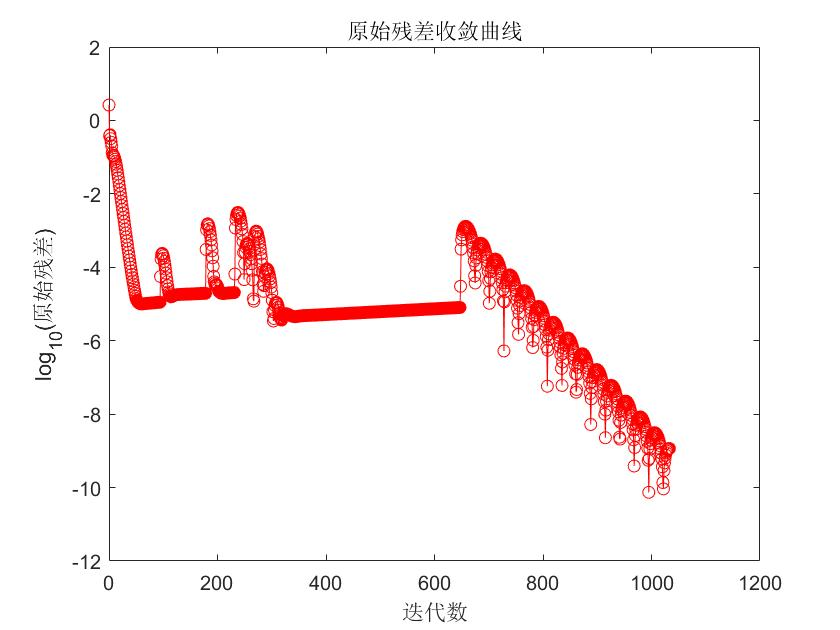
\includegraphics[width=\linewidth]{n4primalres.jpg}
		\end{minipage}}
	\subfigure[对偶残差]{
			\begin{minipage}[b]{.31\linewidth}
				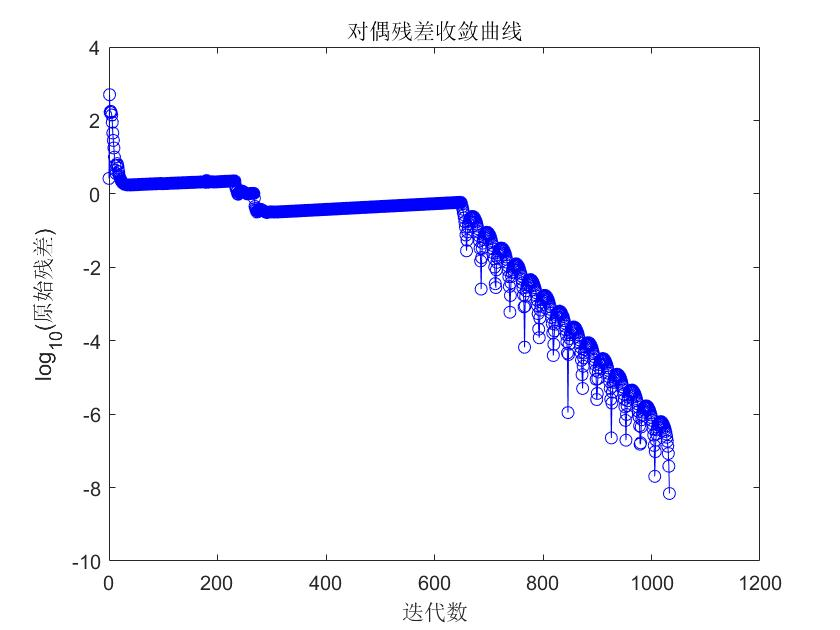
\includegraphics[width=\linewidth]{n4dualres.jpg}
			\end{minipage}}
	\subfigure[目标函数值]{
				\begin{minipage}[b]{.31\linewidth}
					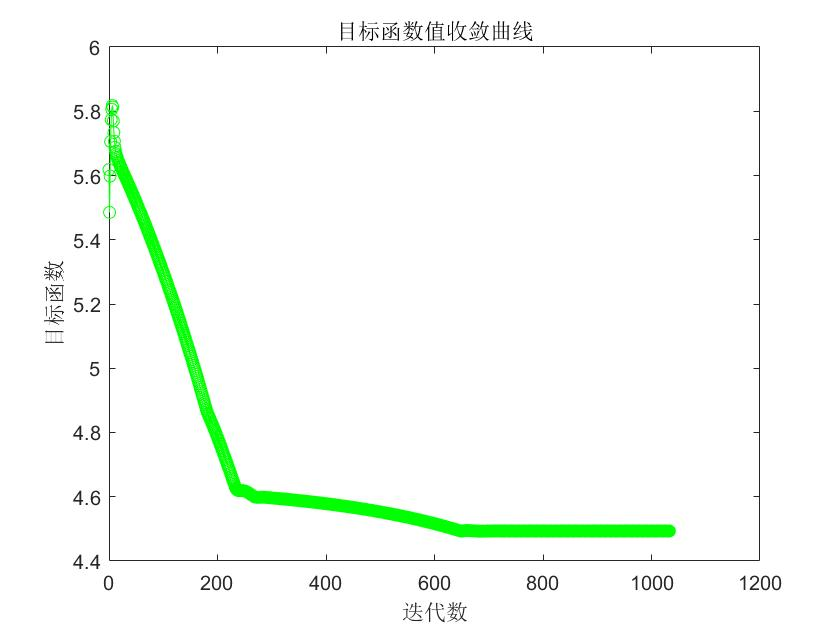
\includegraphics[width=\linewidth]{n4obj.jpg}
				\end{minipage}}
\end{figure}
\begin{center}
	\small\textcolor[rgb]{0,0.25,0.604}{图 1: }$n=4$收敛曲线
\end{center}
\end{frame}

\subsection{松弛因子$\alpha$}
\begin{frame}{数值实验--松弛因子$\alpha$}
$\alpha=0.1,0.2,\ldots,1.0. $
\only<1>{\begin{center}
	\small\textcolor[rgb]{0,0.25,0.604}{表 1: }$n=3$, 不同的松弛因子
\end{center}
\tnewroman
\begin{table}[htbp]
    \centering
    \label{n3alpha}
    \begin{tabular}{c|c|c|c|c}
        \hline
        \multirow{2}{*}{$\alpha$} & \multicolumn{4}{c}{$n=3$}\\\cline{2-5}
          & 迭代数 & 所耗时间 (\tnewroman{s}) & \tnewroman{KKT}违反度 & 目标值\\\hline
        0.1 & \textbf{452} & \textbf{0.0072} & 3.40$\times10^{-9}$ & \textbf{1.1722} \\\hline
        0.2 & 491 & 0.0079 & 8.45$\times10^{-9}$ & \textbf{1.1722} \\\hline
        0.3 & 510 & 0.0088 & 7.07$\times10^{-9}$ & \textbf{1.1722} \\\hline
        0.4 & 517 & 0.0098 & \textbf{2.86$\mathbf{\times10^{-9}}$} & \textbf{1.1722} \\\hline
        0.5 & 503 & 0.0080 & 7.45$\times10^{-9}$ & \textbf{1.1722} \\\hline
        0.6 & 534 & 0.0103 & 7.79$\times10^{-9}$ & \textbf{1.1722} \\\hline
        0.7 & 538 & 0.0093 & 5.69$\times10^{-9}$ & \textbf{1.1722} \\\hline
        0.8 & 525 & 0.0082 & 3.24$\times10^{-9}$ & \textbf{1.1722} \\\hline
        0.9 & 548 & 0.0105 & 8.97$\times10^{-9}$ & \textbf{1.1722} \\\hline
        1.0 & 560 & 0.0097 & 8.02$\times10^{-9}$ & \textbf{1.1722} \\\hline
    \end{tabular}
\end{table}
}
\onslide<2>{\begin{center}
	\small\textcolor[rgb]{0,0.25,0.604}{表 2: }$n=30$, 不同的松弛因子
\end{center}
\tnewroman
\begin{table}[htbp]
    \centering
    \label{n30alpha}
    \begin{tabular}{c|c|c|c|c}
        \hline
        \multirow{2}{*}{$\alpha$} & \multicolumn{4}{c}{$n=30$}\\\cline{2-5}
          & 迭代数 & 所耗时间 (s) & KKT违反度 & 目标值\\\hline
        0.1 & 117886 & 74.7150 & 9.74$\times10^{-7}$ & 26.2298 \\\hline
        0.2 & 69365 & 42.6729 & 8.60$\times10^{-7}$ & 25.8871 \\\hline
        0.3 & 70989 & 43.2812 & 8.88$\times10^{-7}$ & 25.8828 \\\hline
        0.4 & \textbf{65533} & \textbf{40.0219} & 6.46$\times10^{-7}$ & 25.8757 \\\hline
        0.5 & 122029 & 76.4424 & 9.28$\times10^{-7}$ & 25.6165 \\\hline
        0.6 & 112336 & 82.8559 & 9.63$\times10^{-7}$ & 25.6165 \\\hline
        0.7 & 112002 & 70.1342 & 8.81$\times10^{-7}$ & 25.6165 \\\hline
        0.8 & 109121 & 67.5131 & 7.99$\times10^{-7}$ & 25.6165 \\\hline
        0.9 & 113655 & 70.1853 & 8.83$\times10^{-7}$ & 25.6165 \\\hline
        1.0 & 207788 & 129.1006 & \textbf{6.00$\mathbf{\times10^{-7}}$} & \textbf{24.9461} \\\hline
    \end{tabular}
\end{table}}
\end{frame}

%\begin{frame}{数值实验--松弛因子$\alpha$}
%$\alpha=0.1,0.2,\ldots,1.0$.
%\begin{itemize}
%\item 不同的松弛因子可能会影响目标值.
%\item 松弛因子对小型问题不会有多大影响, 但却十分影响大型问题.
%\end{itemize}
%\end{frame}

\subsection{惩罚因子$\beta$}
\begin{frame}{数值实验--惩罚因子$\beta$}
\begin{equation}\left\{\begin{array}{ll}
	\beta=10^2,10^3,10^4,10^5, & n=3,4,5,\\
	\beta=10^3,10^4,10^5, & n=20,\\
	\beta=10^4,10^5, & n=30.
\end{array}\right.\end{equation}\vspace{1em}
\only<1>{\begin{center}
	\small\textcolor[rgb]{0,0.25,0.604}{表 3: }$n=3$, 不同的惩罚因子
\end{center}
\tnewroman
\begin{table}[htbp]
    \centering
    \label{n3beta}
    \begin{tabular}{c|c|c|c|c}
        \hline
        \multirow{2}{*}{$\beta$} & \multicolumn{4}{c}{$n=3$}\\\cline{2-5}
          & 迭代数 & 所耗时间 (s) & KKT违反度 & 目标值\\\hline
        100 & \textbf{224} & \textbf{0.0043} & 5.46$\times10^{-9}$ & \textbf{1.1722}\\\hline
        1000 & 560 & 0.0095 & 8.02$\times10^{-9}$ & \textbf{1.1722}\\\hline
        10000 & 3998 & 0.0647 & \textbf{4.92$\mathbf{\times10^{-9}}$} & \textbf{1.1722}\\\hline
        100000 & 38377 & 0.5818 & 7.68$\times10^{-9}$ & \textbf{1.1722}\\\hline
    \end{tabular}
\end{table}}
\only<2>{\begin{center}
	\small\textcolor[rgb]{0,0.25,0.604}{表 4: }$n=5$, 不同的惩罚因子
\end{center}
\tnewroman
\begin{table}[htbp]
    \centering
    \label{n5beta}
    \begin{tabular}{c|c|c|c|c}
        \hline
        \multirow{2}{*}{$\beta$} & \multicolumn{4}{c}{$n=5$}\\\cline{2-5}
          & 迭代数 & 所耗时间 (s) & KKT违反度 & 目标值\\\hline
        100 & 969 & 0.0465 & 5.00$\times10^{-9}$ & \textbf{2.7741}\\\hline
        1000 & \textbf{860} & \textbf{0.0384} & 9.54$\times10^{-9}$ & \textbf{2.7741}\\\hline
        10000 & 3857 & 0.1698 & \textbf{4.64$\mathbf{\times10^{-9}}$} & \textbf{2.7741}\\\hline
        100000 & 33470 & 1.4344 & 9.47$\times10^{-9}$ & \textbf{2.7741}\\\hline
    \end{tabular}
\end{table}
}
\only<3>{\begin{center}
	\small\textcolor[rgb]{0,0.25,0.604}{表 5: }$n=20$, 不同的惩罚因子
\end{center}
\tnewroman
\begin{table}[htbp]
    \centering
    \label{n20beta}
    \begin{tabular}{c|c|c|c|c}
        \hline
        \multirow{2}{*}{$\beta$} & \multicolumn{4}{c}{$n=20$}\\\cline{2-5}
          & 迭代数 & 所耗时间 (s) & KKT违反度 & 目标值\\\hline
        1000 & \textbf{12122} & \textbf{4.1522} & 9.95$\times10^{-7}$ & \textbf{9.8692}\\\hline
        10000 & 79052 & 26.7695 & \textbf{5.02$\mathbf{\times10^{-7}}$} & \textbf{9.8692}\\\hline
        100000 & 753429 & 255.0805 & 9.98$\times10^{-7}$ & \textbf{9.8692}\\\hline
    \end{tabular}
\end{table}
}
\only<4>{\begin{center}
	\small\textcolor[rgb]{0,0.25,0.604}{表 6: }$n=30$, 不同的惩罚因子
\end{center}
\tnewroman
\begin{table}[htbp]
    \centering
    \label{n30beta}
    \begin{tabular}{c|c|c|c|c}
        \hline
        \multirow{2}{*}{$\beta$} & \multicolumn{4}{c}{$n=30$}\\\cline{2-5}
          & 迭代数 & 所耗时间 (s) & KKT违反度 & 目标值\\\hline
        10000 & \textbf{207788} & \textbf{133.6154} & \textbf{6.00$\mathbf{\times10^{-7}}$} & \textbf{24.9461}\\\hline
        100000 & 2053406 & 1327.5987 & 7.08$\times10^{-7}$ & 24.9542\\\hline
    \end{tabular}
\end{table}
}
\onslide<5>{
\begin{figure}[htbp]
	\centering
	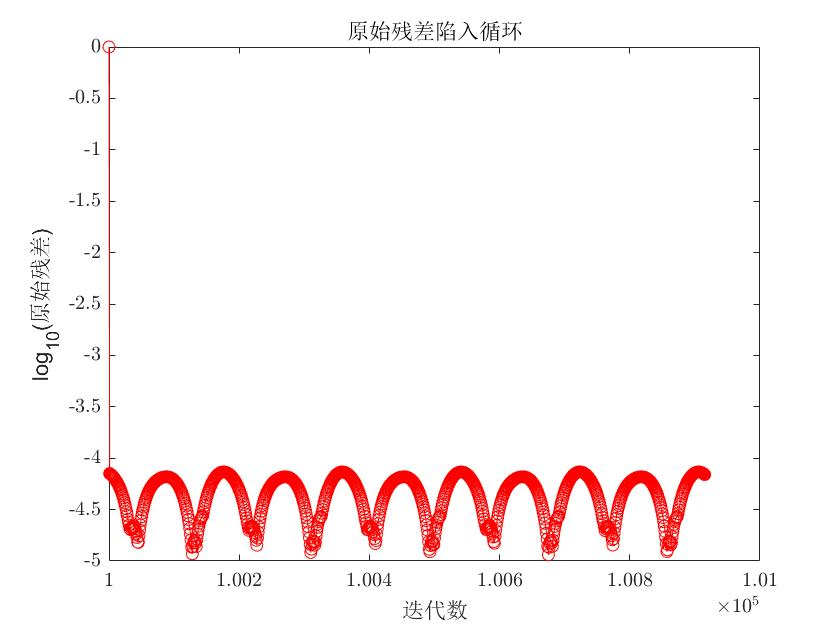
\includegraphics[width=.37\paperwidth]{primalres.jpg}
	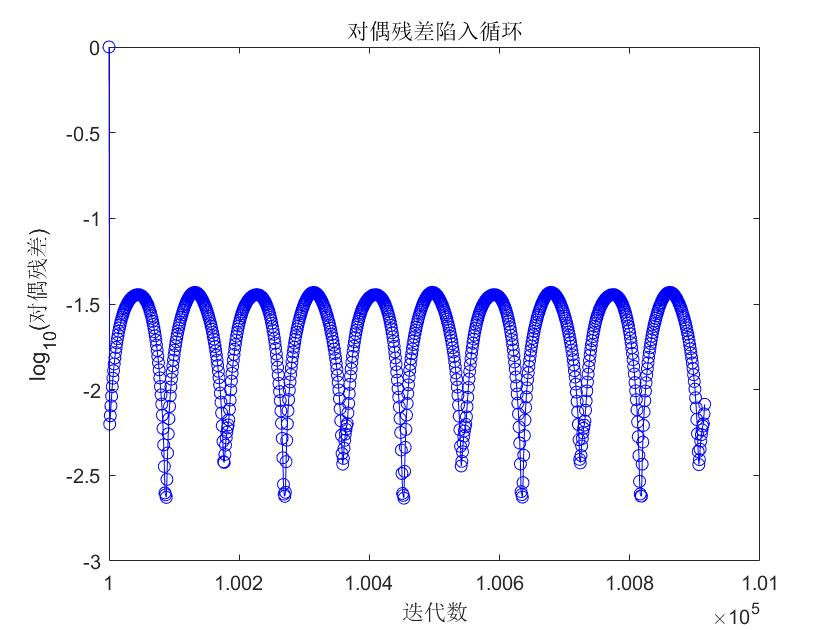
\includegraphics[width=.37\paperwidth]{dualres.jpg}
	\label{loop}
\end{figure}
\begin{center}
	\small\textcolor[rgb]{0,0.25,0.604}{图 2: }$n=30,\beta=10^3$残差陷入循环. 左: 原始残差; 右: 对偶残差
\end{center}
}
\end{frame}

%\begin{frame}{数值实验--惩罚因子$\beta$}
%\begin{itemize}
%\item 惩罚因子需适当选取. 过大减缓算法收敛, 过小可能使算法失效.
%\item 适宜惩罚因子的值域问题维数正相关, 即问题维数越大, 应选取更大的惩罚因子.
%\end{itemize}
%\end{frame}

\subsection{测试问题}
\begin{frame}{数值实验--测试问题}
\begin{itemize}
\item 目的: 表明算法\ref{ADMM}的确可以达到全局最优解.
\item 构造方式: 给定一数对$(p,q):p\ne q,p,q\in\{1,2,\ldots,n\}$, 定义$R$为
\begin{equation}r_{ij}=\left\{\begin{array}{ll}
	1, & i=p,j=q\makebox{或}i=q,j=p,\\
	0, & \makebox{其它}.
\end{array}\right.\end{equation}
$\rho:=\one$. 
\begin{equation}\begin{array}{rl}
	\min\limits_X & 2x_{pq}+2\sum\limits_ix_{ip}x_{iq}\\
	\st & X\one=\rho,X^T\one=\rho,X\ge0,\trace(X)=0.
\end{array}\end{equation}
最优值为\tnewroman0.
\end{itemize}
\end{frame}

\begin{frame}{数值实验--测试问题 (续)}
	$$\begin{array}{rl}
		\min\limits_X & 2x_{pq}+2\sum\limits_ix_{ip}x_{iq}\\
		\st & X\one=\rho,X^T\one=\rho,X\ge0,\trace(X)=0.
	\end{array}$$
	$n=5,10,15,20$, $(p,q)=(3,4)$, $\alpha=1,\beta=10^3,\epsilon=10^{-8}$.\\
	\begin{center}
		\small\textcolor[rgb]{0,0.25,0.604}{表 7: }测试问题, $n=5,10,15,20$
	\end{center}
	\tnewroman
	\begin{table}[H]
		\centering
		\label{test}
		\begin{tabular}{c|c|c|c|c}
			\hline
			$n$ & 迭代数 & 所耗时间 (s) & KKT违反度 & 目标值\\\hline
			5 & 3187 & 0.1536 & 3.00$\times10^{-9}$ & -1.44$\times10^{-11}$\\\hline
			10 & 1447 & 0.1766 & 1.65$\times10^{-9}$ & -4.94$\times10^{-15}$\\\hline
			15 & 2243 & 0.3284 & 2.30$\times10^{-9}$ & 6.54$\times10^{-13}$\\\hline
			20 & 2030 & 0.3299 & 4.53$\times10^{-9}$ & -8.07$\times10^{-13}$\\\hline
		\end{tabular}
	\end{table}
\end{frame}

\subsection{与求解非凸二次规划的算法比较}
\begin{frame}{数值实验--与求解非凸二次规划的算法比较}
\begin{itemize}
\item \tnewroman{MATLAB}内置函数\texttt{fmincon()}, 调用算法\texttt{'sqp','active-set'}求解问题\eqref{original problem matrix form 2}和\eqref{original problem matrix form 1}, 设置停机准则\texttt{ConstraintTolerance}为上文默认值. 在使用算法\ref{ADMM}求解$n=50,60,70,80$的问题, 设置惩罚因子
$$\left\{\begin{array}{ll}
	\beta=10^4, & n=50,60,\\
	\beta=2\times10^4, & n=70,80.
\end{array}\right.$$
\end{itemize}
\end{frame}

\begin{frame}{数值实验--与求解非凸二次规划的算法比较 (续)}
\begin{figure}[H]
	\centering
	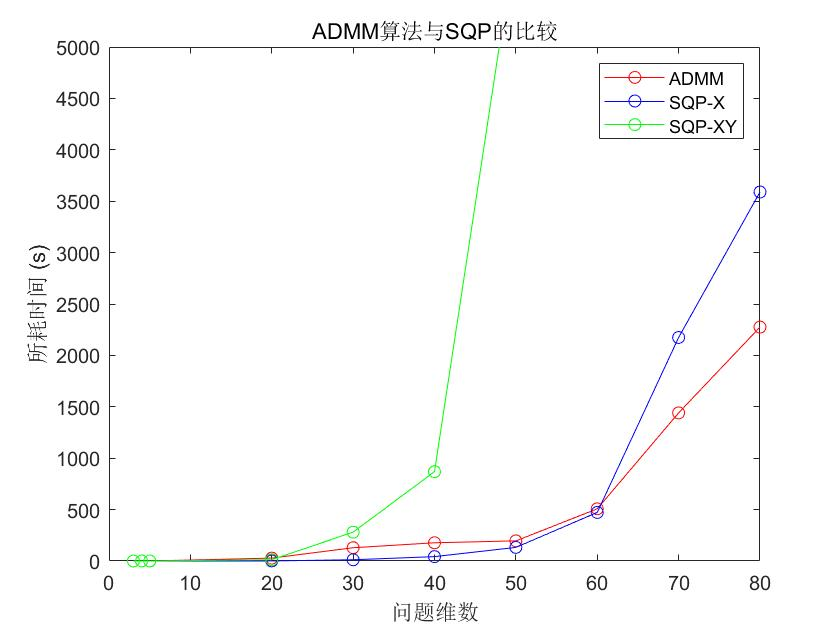
\includegraphics[width=.5\paperwidth]{already.jpg}
	\label{time comparison}
\end{figure}
\begin{center}
		\small\textcolor[rgb]{0,0.25,0.604}{图 3: }算法\ref{ADMM}和\tnewroman SQP运行时间对比
	\end{center}
\textbf{结论}: 对于小型问题, 积极集法和\tnewroman SQP最为便捷; 对于大型问题, 算法\ref{ADMM}更具优势. 算法\ref{ADMM}的缺点在于, 我们需要根据问题的维度不断重新设置惩罚因子$\beta$.
\end{frame}


\section{总结}
\begin{frame}{总结}
\begin{itemize}
\item 针对问题\eqref{original problem matrix form}特殊结构设计了\tnewroman{ADMM}算法.
\item 证明了一定条件下\tnewroman{ADMM}算法\ref{ADMM}收敛到问题\eqref{original problem matrix form}的稳定点.
\item 在随机生成的问题上进行数值实验; 讨论了多个人工给定因子对算法效果的影响; 与求解非凸二次规划的算法做了比较, 得出算法\ref{ADMM}在大型问题上更具优势的结论.
\end{itemize}
\end{frame}
\logo{}
\section*{致谢}
\begin{frame}
\begin{center}
	\Large 感谢聆听!\\[0.5em]
	\small\url{huyukuan2015@tongji.edu.cn}
\end{center}
\end{frame}
\end{document}
